\subsection{Fallschirmjäger}

\subsubsection{Fahrzeuge}
\begin{longtable}{|l|c|c|c|c|} \hline
	Typ 			&		C-130 	&	CH-47 	&	Huron		&		 Mohawk	\\ \hline
	Passagiere 		&		25 		&	25 		&	18 		&		16		\\ \hline
	Min. Sprunghöhe 	&		500m 		&	300m 		&	300m 		&		300		\\ \hline
	Max. Sprunghöhe 	&		6000m 	&	500m 		&	500m 		&		500 		\\ \hline
	Min. Geschwindigkeit& 		200km/h 	&	120km/h 	&	120km/h 	&		120km/h	\\ \hline
	Max. Geschwindigkeit& 		250km/h 	&	150km/h 	&	150km/h 	&		150km/h 	\\ \hline
\end{longtable}

\subsubsection{Sprungvorbereitung}
\paragraph{Kartenvorbereitung} \ \\
\begin{tabular}{p{3cm} p{15cm}}
	
\includegraphics[scale=1]{Endpunkt.png}		&		Sprungzone ab hier beginnt der Loadmaster mit dem Sprung\\
	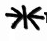
\includegraphics[scale=1]{Treffpunkt.png} 		&		Wendepunkt Pilot übergibt Loadmaster Befehlsgewalt, letzte Vorbereitung vor Sprung\\
	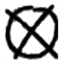
\includegraphics[scale=1]{Aufgabe.png}		&		SZ Sammelzone, ist der Punkt wo sich ein Trupp sammelt, es werden immer 2 Sammelzonen pro Trupp bestimmtl \\
	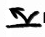
\includegraphics[scale=1]{LZ.png}			&		LZ Landezone, ist der Punkt wo sich alle Truppen sammeln \\
\end{tabular}

\paragraph{Materialvorbereitung/Aufsitzen}  \ \\

	\begin{itemize}
		\item Rucksack auf den Bauch schnallen 
		\item  Fallschirm aus der speziellen Kiste entnehmen
		\item  im Trupp vor der Maschine aufstellen; der Trupp, der als letztes springt, steigt als erstes ein; der Loadmaster ist der letzte der einsteigt
		\item im Fahrzeug selbstständig und ohne Funkbestätigung auf die SR 200 wechseln; Sprungfrequenz
		\item  Truppführer meldet aufsitzen auf der SR 200
	\end{itemize}

	\begin{flushright}
		Merke: >>Der Erste wird der Letzte sein.<< 
	\end{flushright}

\subsubsection{Loadmaster}

	Der Loadmaster hat die Aufgabe den Absprung zu koordinieren, darunter fällt z.B. wer springt zu welcher Zeit. Es wird nur auf sein Kommando gesprungen. \\

\paragraph{Teil der Truppe} \ \\
	Die Rolle des Loadmasters wird von ein Mitglied des zuletzt springenden Trupps wahrgenommen. Der Loadmaster springt immer als letztes ab, egal welche Position er im Trupp hat. \\

\paragraph{Teil des Fahrzeugteams} \ \\
	Die Rolle des Loadmaster wird von einem 3. Mann im Fahrzeug wahrgenommen. Dieser springt am Ende nicht ab, sonder verbleibt im Fahrzeug. \\

\subsubsection{Der Sprung}

\paragraph{empfohlene Sprunghöhen} \ \\
\begin{longtable}{|l|c|c|c|c|} \hline
	Typ 			&		C-130 	&	CH-47 	&	Huron		&		 Mohawk	\\ \hline
	Höhe	[m]		&		500, 1000, 6000 & 300, 500	&	300, 500	&		300, 500	\\ \hline
\end{longtable}

\paragraph{Verhalten beim Sprung} \ \\
	Bei einer Sprunghöhe von 300 - 1000 m wird der Fallschirm sofort nach verlassen des Fahrzeugs geöffnet. \\
	Bei einer Sprunghöhe von 6000 m wird zwischen HALO und HAHO unterschieden \\
	Beim HALO ( High Altitude – Low Opening dt. große Höhe – niedrige Öffnung) wird der Fallschirm ab einer Höhe von 1000m geöffnet. \\
	Beim HAHO ( High Altitude – High Opening dt. große Höhe – hohe Öffnung) wird der Fallschirm sofort nach verlassen des Fahrzeuges geöffnet. \\

\subsubsection{Der Flug}
Es dürfen keine Rauch-, Leucht- oder ähnliche Körper am Mann gezündet werden. \\
\paragraph{6000m} \ \\
	HALO	\\
	Während des gesamten Fluges ist die maximal Geschwindigkeit von 54km/h zuhalten. Zum navigieren ist zu empfehlen sich an seinen Vordermann zuhalten. \\
	HAHO \\
	Während des gesamten Fluges ist die maximal Geschwindigkeit von 54km/h zuhalten. Zum navigieren ist zu empfehlen sich an seinen Vordermann zuhalten. \\

\paragraph{300-1000m} \ \\
	Während des gesamten Fluges ist die maximal Geschwindigkeit von 54km/h zuhalten. Zum navigieren ist zu empfehlen sich an seinen Vordermann zuhalten. \\

\subsubsection{Die Landung}
	\begin{itemize}
		\item beginnt ab einer Höhe von 50m; ab da beträgt die maximal Geschwindigkeit 30km/h,
		\item 20m vor der Landung auf mindestens 20km/h bremsen,
		\item sollte mit 10km/h oder weniger Erfolgen; um Verletzungen zu vermeiden.
	\end{itemize}

\subsubsection{Sammeln}
	\begin{itemize}
		\item nach der Landung wird über den Truppfunk das erfolgreiche landen durchgegeben
		\item eigenständig zur ersten Sammelzone bewegen; dafür sind 5min vorgesehen
		\item wenn alle angekommen dann zur zweiten Sammelzone bewegen; sollten nicht alle zur ersten Sammelzone finden bzw. sich nach der Landung nicht melden wird nach den 5min nach den vermissten Kameraden gesucht
		\item beim erreichen der zweiten Sammelzone ist der Fallschirmsprung abgeschlossen
	\end{itemize}
	